\documentclass[11pt]{article}
\usepackage{tikz}
\usetikzlibrary{arrows.meta,positioning}
\usepackage{tabularx}
\usepackage{amsmath,amssymb,bm,graphicx,booktabs,hyperref,geometry}
\geometry{margin=1in}
\hypersetup{colorlinks=true, linkcolor=blue, citecolor=blue, urlcolor=blue}




\title{\textbf{Paper B-11: Computational Architecture:\\ A Constraint-Driven Flux Dynamics (CDFD) Perspective}}
\author{Steve Bico Mujjabi, MD\\
\small Independent Researcher\\
\small Founder, Vura Labs\\
\small Kampala, Uganda\\
\small ORCID: 0009-0001-0556-5516}
\date{May 2026}


\newcommand{\EarthSuppPath}{Part\_A\_Earth\_Systems/supplementary/supplementary\_earth\_}
\newcommand{\EngSuppPath}{Part\_B\_Engineered\_Systems/supplementary/supplementary\_eng\_}
\newcommand{\SocSuppPath}{Part\_C\_Socioeconomic\_Systems/supplementary/supplementary\_soc\_}
\newcommand{\DomainSuppPath}{Part\_D\_Domain\_Applications/supplementary/supplementary\_dom\_}
\begin{document}

\maketitle
\newpage


\begin{abstract}
In this paper we apply Adaptive Flux Limitation (AFL) to computer architecture, modelling
instruction throughput as constrained transport governed by the potential $\Phi$ (instruction
retirement rate, FLOP/s), with multi-dimensional constraint $C = (C_{mem}, C_{pwr}, C_{IPC})$
encoding memory bandwidth, thermal power budget, and instruction-level parallelism limits.
The effective $\Psi_s^* = J/C_{eff}$ where $C_{eff} = \min(C_{mem}, C_{pwr}, C_{IPC})$ classifies
processor states: memory-bound, power-bound, or IPC-bound.

We model the hypothesis that roofline performance models, cache hierarchy design, heterogeneous chip
architecture (CPUs + GPUs + NPUs), and dark-silicon management emerge naturally from AFL
multi-wall dynamics. Dennard scaling failure is recast as $C_{pwr}$ wall formation; modern
chiplet design is AFL constraint diversification.

\textbf{Status: Inferred from AFL first principles; quantitative predictions are hypothesis-level.}\\
\textbf{Series tag: Eng-B11}
\end{abstract}

\section*{Symbol Conventions}

\noindent\textbf{CDFD/AFL Part IV symbol convention.}
\begin{center}
{\small
\begin{tabular}{p{0.15\linewidth}p{0.34\linewidth}p{0.41\linewidth}}
\hline
Symbol & Part IV meaning & Cross-domain reading \\
\hline
$\Phi$ & Driving flux or throughput & Energy, matter, signal, capital, information, traffic, force, or biological load entering a system \\
$C$ & Active constraint or capacity burden & Bottleneck, resistance, boundary, scarcity, toxicity, regulation, topology, latency, or load-bearing limit \\
$S$ & Responsiveness or adaptive surface & The system's ability to reconfigure, buffer, route, repair, learn, or preserve function under changing load \\
$M_s$ & Structural memory & Stored damage, hysteresis, inherited topology, institutional memory, trained weights, ecological legacy, or retained state \\
$\Psi_s$ & Adaptive operating ratio $(\Phi/C)\cdot S\cdot M_s$ & Local bookkeeping gauge for constrained operation, overload, recovery, or regime change; not a universal constant \\
$\Lambda$ & Life Number or capstone surplus ratio where explicitly defined & Reserved for Part II-derived life-number notation or synthesis-level surplus measures, never an undefined decoration \\
\hline
\end{tabular}
}
\end{center}

\noindent\textbf{Greek-symbol convention.}
\begin{center}
{\small
\begin{tabular}{p{0.15\linewidth}p{0.34\linewidth}p{0.41\linewidth}}
\hline
Symbol & Local role & Interpretation rule \\
\hline
$\alpha$ & Accumulation or reinforcement coefficient & Sets how fast a pathway, constraint, habit, cascade, or retained structure grows under load \\
$\beta$ & Relaxation, decay, clearance, or washout coefficient & Sets loss, recovery, damping, forgetting, degradation, or return toward baseline \\
$\gamma$ & Coupling, diffusion, redistribution, or transfer coefficient & Sets spread across nodes, layers, tissues, markets, infrastructures, media, or physical phases \\
$\delta,\epsilon$ & Perturbation, tolerance, small offset, or numerical guard & Used only as local thresholds, stability margins, measurement tolerances, or stress increments \\
$\eta,\lambda,\mu,\nu$ & Efficiency, rate, baseline, intensity, or frequency terms & Meaning is fixed by the equation, subscript, and domain-specific proxy in the paragraph where the term appears \\
$\rho,\sigma,\tau,\phi$ & Density/correlation, variability/noise, time-scale, phase, or field terms & Local coefficients only; subscripts bind them to the named pathway, domain, or experiment \\
$\Omega,\Lambda$ & Domain/state space; Life Number where defined & $\Omega$ names a modeled state space; $\Lambda$ carries life-number or synthesis notation only when the paper defines it \\
\hline
\end{tabular}
}
\end{center}


\section{Series Context}

Part I sets the flow--constraint language used here \cite{MujjabiPartI2026}. Part II develops the Life Number and the origins-of-life use of the same notation \cite{MujjabiPartII2026}. Part III applies AFL to biology and medicine \cite{MujjabiPartIII2026}. Part IV \cite{MujjabiPartIV2026}, DOI \url{https://doi.org/10.5281/zenodo.20395901}, is the cross-domain stress test: it asks where the notation clarifies measurement, and where it becomes only a metaphor.

\section{Introduction}


\subsection{The Mujjabi Universal Capacity Law}
Building directly upon the Fundamental Physics (Part I) \cite{MujjabiPartI2026}, the \textbf{Mujjabi Universal Capacity Law} proposes that across all scales---from black hole event horizons to global financial markets and power grids---driving high flux ($\Phi$) against a rigid topological constraint ($C$) can drive system saturation. When $\Phi/C$ approaches critical thresholds, the system does not scale linearly; it undergoes a topological phase transition.

\subsection{The Mujjabi Universal Memory Law}
The \textbf{Mujjabi Universal Memory Law} frames persistent systemic collapse. When a complex network fails to clear its structural memory ($M_s$) and its relaxation parameter decays ($\tau_{relax} \to \infty$), temporary stressors become permanent rigidities. This is the proposed CDFD mechanism behind ecological death, economic depressions, and infrastructural gridlock.


Modern processors contain $>10^{10}$ transistors operating at $>10^9$ Hz, yet practical
throughput is limited by three architectural constraints that have converged to form permanent
performance ceilings. These ``walls'' are among the most consequential engineering challenges
in computer science:
\begin{enumerate}
    \item \textbf{Memory wall}: DRAM bandwidth grows at $\sim$26\%/year while CPU performance
          grew at $\sim$52\%/year (through 2004), creating an ever-widening gap;
    \item \textbf{Power wall}: Dennard scaling broke down around 2005; frequency can no longer
          increase without thermal runaway (``dark silicon'');
    \item \textbf{IPC wall}: instruction-level parallelism (ILP) extractable by out-of-order
          execution saturates at $\sim$4--6 IPC for most workloads.
\end{enumerate}

AFL unifies these three walls as a multi-dimensional constraint system: processor throughput
$J$ is jointly bounded by three independent $C$ values, and the effective constraint is
$C_{eff} = \min(C_{mem}, C_{pwr}, C_{IPC})$ --- the weakest wall determines performance.
This provides a single $\Psi_s^* = J/C_{eff}$ diagnostic for architectural bottleneck ($\Psi_s > 1$ lock state) identification.

\section{Core Hypothesis}

\begin{center}
\textit{
Computational throughput in processor architecture is governed by a multi-dimensional AFL system
in which three converging constraints (memory bandwidth, power budget, instruction parallelism)
jointly bound instruction retirement rate, with heterogeneous chip design representing the
AFL strategy for constraint diversification across varied workload types.
}
\end{center}

AFL architecture hypothesis: the roofline performance model is an AFL two-constraint model
($C_{mem}$ and $C_{peak-FLOP}$), and the ``roofline knee'' is the AFL $\Psi_s^* = 1$ operating
point where compute and memory constraints are balanced. Modern performance engineering
seeks workloads where $\Psi_s^* \approx 1$ on the compute roofline rather than the memory roofline.
\textbf{Status: Hypothesis; roofline model provides direct structural correspondence.}

\section{Computational Potential Field}

We define the generalised processor potential:
\begin{equation}
\Phi = \text{instruction retirement rate} = \text{IPC} \times f
\end{equation}
where IPC is instructions per cycle and $f$ is clock frequency. The AFL transport equation
governs how $\Phi$ flows through the processor pipeline:
\begin{equation}
J = -\frac{1}{C_{eff}}\nabla \Phi
\end{equation}
where $C_{eff}$ encodes the binding constraint at any given workload.

\section{The Three-Wall AFL System}

\subsection{Memory Wall: $C_{mem}$}

Memory bandwidth constraint:
\begin{equation}
C_{mem} = \frac{\text{Arithmetic Intensity}}{\text{Peak Memory Bandwidth}} = \frac{FLOP/byte}{BW_{peak}}.
\end{equation}

A workload is memory-bound when $J_{compute} > C_{mem}$: the processor can perform more
operations than the memory subsystem can supply data for. AFL prediction: memory-bound
workloads have $\Psi_{s,mem} > 1$; they waste compute cycles waiting for data.

Cache hierarchy is AFL constraint reduction: L1 cache reduces effective $C_{mem}$ for data
with high temporal locality by a factor of $\sim100$ (DRAM vs.\ L1 latency ratio).

\subsection{Power Wall: $C_{pwr}$}

Thermal power constraint:
\begin{equation}
C_{pwr} = \frac{P_{TDP}}{P_{per-transistor}} = \frac{P_{TDP}}{\alpha CV^2 f},
\end{equation}
where $P_{TDP}$ is thermal design power, $C$ (here capacitance) is switching capacitance per
transistor, $V$ is supply voltage, $f$ is frequency.

Dennard scaling: through 2004, $V \propto f$ kept $P_{per-transistor} \propto f^{-2}$, so
scaling $f$ preserved $P_{total}$. When $V$ could not decrease further (leakage current), $P_{pwr}
\propto f^3$ and scaling ceased. AFL interpretation: $C_{pwr}$ wall formed when Dennard scaling
exhausted the adaptive mechanism ($\beta_{Dennard} \to 0$).

\textbf{Dark silicon}: when only a fraction $f_{active}$ of transistors can be active simultaneously
at design power, $J_{compute} = f_{active} \cdot J_{peak}$. AFL $\Psi_{s,pwr} = J_{peak}/(f_{active}
C_{pwr})$: dark silicon is the AFL response to power-wall constraint --- reduce $J_{active}$
to maintain $\Psi_{s,pwr} \leq 1$.

\subsection{IPC Wall: $C_{IPC}$}

Instruction-level parallelism constraint:
\begin{equation}
C_{IPC} = \frac{1}{ILP_{extractable}}
\end{equation}
where $ILP_{extractable}$ is the average instruction-level parallelism available in the
instruction stream. Out-of-order execution, branch prediction, and speculative execution
increase $ILP_{extractable}$, reducing $C_{IPC}$.

Amdahl's law at the instruction level: sequential data dependencies (RAW hazards) impose
irreducible $C_{IPC}$. Modern OOO processors extract $\sim$4--6 IPC for integer workloads;
the IPC wall is the AFL sequential-fraction constraint at microarchitectural scale.

\section{Conservation Dynamics}

Processor throughput obeys conservation:
\begin{equation}
\frac{\partial \Phi}{\partial t} + \nabla \cdot J = S
\end{equation}
where $S$ represents instruction supply (from the instruction cache and decoder) and $J$
represents instruction retirement (completed execution). The pipeline is the AFL transport
medium; the reorder buffer (ROB) is the AFL queue.

\section{Adaptive Constraint Dynamics}

Architectural constraints evolve dynamically:
\begin{equation}
\frac{dC_{eff}}{dt} = \alpha |J| - \beta C_{eff}
\end{equation}
where $\alpha$ governs workload-induced constraint stress (high throughput fills ROB, causes
branch mispredictions, increases cache pressure) and $\beta$ governs microarchitectural
recovery (branch predictor warms up, prefetcher learns access patterns, TLB reloads).

Physical mechanisms:
\begin{itemize}
    \item \textbf{Branch misprediction}: wrong-path speculation fills ROB; recovery flushes
          pipeline (transient $J \to 0$, $C$ spikes);
    \item \textbf{Cache miss cascade}: L1 miss $\to$ L2 miss $\to$ L3 miss $\to$ DRAM: each level
          increases effective $C_{mem}$ by $\sim10\times$;
    \item \textbf{TLB miss}: virtual-to-physical address translation miss requires page-walk,
          adding $\sim$100 cycle penalty to effective $C$;
    \item \textbf{Hardware prefetcher}: learns memory access patterns, reducing effective
          $C_{mem}$ by prefetching data before it is needed ($\beta$ mechanism).
\end{itemize}

\subsection{Adaptive Surface Dynamics: Memory and Responsiveness}

The operating ratio $\Psi_s^*$ is mediated by adaptive surface components:
\begin{equation}
\Psi_s^* = (\Phi/C) \cdot S \cdot M_s
\end{equation}
where $S$ (Surface Responsiveness) and $M_s$ (Surface Memory) evolve as:
\begin{align}
\frac{dS}{dt} &= \kappa_s (\Psi_s^* - S) \\
\frac{dM_s}{dt} &= \Phi S - d_m M_s
\end{align}
These components represent the homeostatic capacity of the system to regulate its own operating ratio through memory and responsiveness.

\section{Flux--Constraint Number}

\begin{equation}
\Psi_s^* = \frac{J}{C_{eff}} = \frac{J}{\min(C_{mem}, C_{pwr}, C_{IPC})}
\end{equation}

\subsection{Memory-Bound Regime ($C_{mem}$ dominates)}

Workload has low arithmetic intensity; processor waits for data. Memory-bound workloads:
streaming operations (memcpy, matrix transpose), sparse linear algebra, large graph traversal.
AFL $\Psi_{s,mem} > 1$: processors can compute faster than memory can supply.

\subsection{Compute-Bound Regime ($C_{IPC}$ or $C_{pwr}$ dominates)}

Workload has high arithmetic intensity; memory latency is hidden. Dense matrix multiplication
(GEMM), FFT on cached data, neural network forward pass on GPU. AFL $\Psi_{s,mem} < 1$:
memory is not the bottleneck ($\Psi_s > 1$ lock state); compute is the limit.

\subsection{Thermally Limited Regime ($C_{pwr}$ dominates)}

All transistors operational but power budget exhausted; frequency must be reduced below rated
speed. Mobile processors and sustained HPC workloads operate in this regime. AFL $\Psi_{s,pwr}
\to 1$: processor executes at thermal steady-state.

\section{The Roofline Model as Two-Wall AFL}

The Roofline performance model (Williams, Waterman, Patterson 2009) plots:
\begin{align}
\text{Attainable GFLOP/s} &= \min(P_{peak}, B_{peak} \times I)
\end{align}
where $I$ is arithmetic intensity (FLOP/byte), $P_{peak}$ is peak compute, $B_{peak}$ is
peak bandwidth. This is the AFL two-wall model:
\begin{align}
J &= \min\left(\frac{\Phi}{C_{mem}}, \frac{\Phi}{C_{IPC}}\right)\\
\Psi_s^* &= \frac{J}{\min(C_{mem}, C_{IPC})}
\end{align}

The roofline ``knee'' at $I_{knee} = P_{peak}/B_{peak}$ is the AFL $\Psi_s^* = 1$ balanced point.
Optimising code for the roofline model is AFL constraint balancing: raise $I$ (increase
compute per byte) until $\Psi_{s,mem} = \Psi_{s,IPC} = 1$.

\section{Cache Hierarchy as AFL Constraint Reduction}

Cache hierarchy reduces effective $C_{mem}$:
\begin{equation}
C_{mem,eff} = h_1 C_{L1} + (1-h_1)h_2 C_{L2} + (1-h_1)(1-h_2)C_{DRAM}
\end{equation}
where $h_1, h_2$ are L1, L2 hit rates and $C_{L1} \ll C_{L2} \ll C_{DRAM}$.

AFL cache design principle: keep $C_{L1}$ small enough that $\Psi_{s,L1} < 1$ for the
temporal-locality working set; $C_{L2}$ for the spatial-locality working set. Cache size
is AFL constraint buffer sizing.

\section{Heterogeneous Architecture as AFL Constraint Diversification}

Modern chips combine multiple processor types:
\begin{align}
\text{CPU} &\to \text{low-latency sequential workloads}\\
\text{GPU} &\to \text{high-throughput parallel workloads}\\
\text{NPU/TPU} &\to \text{matrix-multiplication workloads}
\end{align}

This is AFL constraint diversification: each accelerator has different $(C_{mem}, C_{pwr},
C_{IPC})$, and the heterogeneous system routes workloads to the accelerator where $\Psi_s^* \approx 1$:
\begin{equation}
\text{optimal routing: } J_{workload} \to \text{accelerator}^* = \arg\min_k \Psi_{s,k}
\end{equation}

GPUs have $C_{IPC,GPU} \ll C_{IPC,CPU}$ (massively parallel), but $C_{mem,GPU} \sim C_{mem,CPU}$
per core. Matrix operations with high arithmetic intensity ($I > 100$ FLOP/byte) have
$\Psi_{s,GPU} \approx 1$ (compute-bound on GPU) while $\Psi_{s,CPU} \gg 1$ (memory-bound on CPU).

\section{Chiplet Architecture}

Modern chiplet design (AMD EPYC, Apple M-series, Intel Meteor Lake) disaggregates monolithic
die into compute tiles, memory tiles, and I/O tiles. This is AFL modularisation:
\begin{equation}
C_{eff,chiplet} < C_{eff,monolithic}
\end{equation}
because each chiplet is optimised for its constraint type, and inter-chiplet interconnects
(UCIe, HBM stacking) are designed for the specific $J$ between chiplet types.

\section{Spatial Self-Organization}

Processor microarchitecture self-organises into execution hierarchies (pipeline stages), throughput
corridors (critical paths), caching hubs (shared L3), and adaptive resource pools (ROB, issue
queue). This organisation minimises effective execution constraint while maximising instruction
retirement throughput.

AFL-PDE simulations (\texttt{supplementary\_eng\_11.py}) model three-wall AFL: $\Psi_{s,mem}$,
$\Psi_{s,pwr}$, $\Psi_{s,IPC}$ evolve under a synthetic workload trace, showing which wall is
binding at each time step and how microarchitectural optimisations shift the binding constraint.

\section{Predictions}

\begin{enumerate}
    \item \textbf{Roofline knee}: optimal arithmetic intensity $I^* = P_{peak}/B_{peak}$;
          AFL confirms this is the $\Psi_{s,mem} = \Psi_{s,IPC}$ balance point.
    \item \textbf{Dark silicon fraction}: fraction of active transistors $f_{active} = P_{TDP}/
          (\alpha_{sw} C V^2 f N)$; AFL predicts $f_{active}$ scales inversely with frequency.
    \item \textbf{Cache sizing}: optimal L1 cache size equals temporal working-set size;
          AFL predicts $h_1 = 1 - C_{L2}/C_{DRAM}$ at optimal sizing.
    \item \textbf{Heterogeneous routing}: workloads with $I > I^* _{GPU}$ should route to GPU;
          AFL predicts routing threshold from accelerator roofline parameters.
    \item \textbf{Chiplet benefit}: chiplet disaggregation reduces $C_{eff}$ by $\delta C \propto
          N_{tiles} \cdot \Delta C_{specialisation}$; AFL quantifies chiplet advantage.
\end{enumerate}

\textbf{Status: Predictions 1--2 consistent with established computer architecture results;
predictions 3--5 are AFL extensions requiring microarchitectural measurement.}

\section{Computational Interpretation}

The companion script \texttt{supplementary\_eng\_11.py} implements AFL three-wall architecture:
\begin{itemize}
    \item workload trace with varying arithmetic intensity $I(t)$;
    \item three constraint channels: $C_{mem}(I, BW)$, $C_{pwr}(f, V, N)$, $C_{IPC}(ILP)$;
    \item $\Psi_{s,eff} = J/\min(C_{mem}, C_{pwr}, C_{IPC})$ plotted vs.\ time;
    \item roofline: performance vs.\ intensity curve with memory and compute bounds;
    \item outputs: three-wall $\Psi_s^*$ timeline, roofline plot, cache sizing recommendation.
\end{itemize}

\section{Discussion}

AFL unifies computer architecture under a three-wall multi-constraint framework. The memory
wall, power wall, and IPC wall are three independent AFL constraints; the roofline model is
two-wall AFL; heterogeneous architecture is AFL constraint diversification; chiplets are AFL
modularisation. The AFL architectural design principle: minimise $C_{eff} = \min(C_{mem},
C_{pwr}, C_{IPC})$ by balancing across all three constraints simultaneously.

The key AFL insight: architectural optimisation should target $\Psi_{s,mem} = \Psi_{s,pwr} =
\Psi_{s,IPC} = 1$ simultaneously (all walls equally binding), which maximises efficient
utilisation of all resources. Modern heterogeneous designs approach this ideal by routing
each workload type to the accelerator where its specific wall is the binding constraint.



\section{Measurement Layer}

The first job in any domain is to choose proxies before drawing conclusions. $\Phi$ may be a rate of material, energy, information, capital, or signal flow. $C$ is the bottleneck that slows or redirects that flow. $S$ measures the system's ability to reconfigure under stress, and $M_s$ records the past load that still changes present behavior. A useful application gives those four terms observable definitions, a time scale, and a failure condition. If a standard domain model explains the same data more cleanly, the CDFD/AFL mapping should give way.

\subsection{Current Runtime Diagnostic: Universal Network Cascade}
The release-local discovery script keeps this paper tied to the current CDFD Runtime \cite{CDFDRuntime2026}, including RK4 field updates, surface dynamics, structural-memory diffusion, and a finite-value audit. In the 2026-06-04 runtime pass, the localized hub-drive stress test ended with hub $\Psi_s=5.21$, peak network $\Psi_s=5.21$, 21 nodes above $\Psi_s>1.5$, and 37 maximum memory-locked nodes. I treat those numbers as a runtime sanity check and as a target for later domain measurement, not as a substitute for field data.


% BEGIN PART IV MAJOR UNIVERSAL UPGRADE
\section{Major Universal Upgrade: Mechanism, Scale, and Tests}

\subsection{Observable Translation}

The paper-specific translation begins with an observable chain rather than a
verbal analogy. For Computational Architecture, the proposed drive is instructions, data, memory requests, and synchronization.
The active limitation is memory bandwidth, dependencies, energy, latency, and physical layout. Responsiveness is carried by
parallelism, caching, speculation, scheduling, and specialization, while retained state is represented by
architectural state, compiler choices, cache history, and accumulated heat. The outcome to explain is throughput, latency, energy efficiency, and correctness.

\begin{table}[htbp]
\centering
\small
\caption{Operational CDFD/AFL map for Paper B-11.}
\begin{tabularx}{\textwidth}{|l|X|X|}
\hline
\textbf{Term} & \textbf{Paper-specific observable meaning} & \textbf{Measurement question} \\
\hline
$\Phi$ & instructions, data, memory requests, and synchronization & What rate, load, gradient, or demand enters the focal system? \\
\hline
$C$ & memory bandwidth, dependencies, energy, latency, and physical layout & Which measured bottleneck limits transfer, function, or recovery? \\
\hline
$S$ & parallelism, caching, speculation, scheduling, and specialization & Which process changes effective capacity or reroutes the load? \\
\hline
$M_s$ & architectural state, compiler choices, cache history, and accumulated heat & Which retained state makes equal present loads produce different futures? \\
\hline
$Y$ & throughput, latency, energy efficiency, and correctness & Which outcome is predicted out of sample, with uncertainty? \\
\hline
\end{tabularx}
\end{table}

\begin{figure}[htbp]
\centering
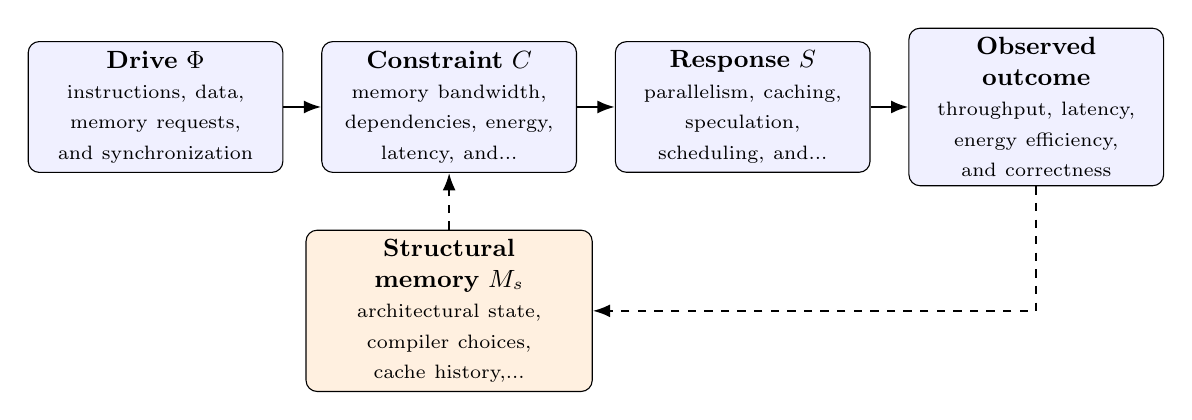
\begin{tikzpicture}[
    node distance=0.48cm,
    every node/.style={font=\small},
    box/.style={draw, rounded corners, align=center, minimum height=1.45cm, text width=3.0cm, fill=blue!6},
    memory/.style={draw, rounded corners, align=center, minimum height=1.25cm, text width=3.4cm, fill=orange!12},
    flow/.style={-{Latex[length=2.2mm]}, thick},
    feedback/.style={-{Latex[length=2.2mm]}, thick, dashed}
]
\node[box] (drive) {\textbf{Drive $\Phi$}\\\scriptsize instructions, data, memory requests, and synchronization};
\node[box, right=of drive] (constraint) {\textbf{Constraint $C$}\\\scriptsize memory bandwidth, dependencies, energy, latency, and...};
\node[box, right=of constraint] (response) {\textbf{Response $S$}\\\scriptsize parallelism, caching, speculation, scheduling, and...};
\node[box, right=of response] (outcome) {\textbf{Observed outcome}\\\scriptsize throughput, latency, energy efficiency, and correctness};
\node[memory, below=0.72cm of constraint] (memory) {\textbf{Structural memory $M_s$}\\\scriptsize architectural state, compiler choices, cache history,...};
\draw[flow] (drive) -- (constraint);
\draw[flow] (constraint) -- (response);
\draw[flow] (response) -- (outcome);
\draw[feedback] (outcome.south) |- (memory.east);
\draw[feedback] (memory.north) -- (constraint.south);
\end{tikzpicture}
\caption{Paper B-11 observable CDFD/AFL architecture for Computational Architecture. Solid arrows give the proposed forward chain; dashed arrows make history-dependent feedback explicit.}
\label{fig:b11-architecture}
\end{figure}

\subsection{Minimal Coupled Model}

A paper-level model must separate throughput, constraint accumulation, response,
and history. One deliberately minimal form is
\begin{align}
Y(t) &= \frac{\Phi(t)S(t)}{\epsilon + C(t)}, \\
\frac{dC}{dt} &= \alpha \Phi(t) - \beta S(t)C(t) + \gamma \mathcal{L}C(t), \\
\frac{dM_s}{dt} &= \eta C(t) - \mu M_s(t), \\
\Psi_s(t) &= \frac{\widehat{\Phi}(t)}{\epsilon+\widehat{C}(t)}\,
             \widehat{S}(t)\,[1+\omega\widehat{M_s}(t)] .
\end{align}
Here $Y$ is the measured output, $\epsilon>0$ prevents a singular denominator,
$\mathcal{L}$ is a spatial or network coupling operator, and hats denote
explicitly normalized variables. The sign and magnitude of $\omega$ must be
estimated: memory can preserve useful organization or amplify damage. No fixed
threshold is universal before the variables, normalization, and observation
scale are declared.

For this paper, the hypothesized causal sequence is specific. A change in
instructions, data, memory requests, and synchronization arrives faster than parallelism, caching, speculation, scheduling, and specialization can compensate.
This raises or redistributes memory bandwidth, dependencies, energy, latency, and physical layout. If the load persists,
the retained state encoded by architectural state, compiler choices, cache history, and accumulated heat changes the next response, so a later event of equal
magnitude can produce a different trajectory in throughput, latency, energy efficiency, and correctness. The
scientific task is to estimate that sequence against the best ordinary model of
the domain, not merely to redescribe the outcome after it occurs.

\subsection{Cross-Scale Universality Without Mechanistic Erasure}

For the engineered systems family, the universal comparison is between demand, designed capacity, feedback control, dependency topology, and accumulated technical state. The strongest engineering use is prospective: the mapping must identify a bottleneck, a control action, or a recovery signature before the failure occurs. \cite{BarabasiAlbert1999,WattsStrogatz1998,Shannon1948,BakTangWiesenfeld1987}
The CDFD programme is cumulative: Part I supplies the flow--constraint
foundation \cite{MujjabiPartI2026}; Part II asks when maintained throughput
supports persistent organized states \cite{MujjabiPartII2026}; Part III
develops adaptive limitation and biological memory \cite{MujjabiPartIII2026};
and Part IV \cite{MujjabiPartIV2026} tests how much of that architecture
survives translation. The CDFD Runtime \cite{CDFDRuntime2026} supplies a
reproducible numerical stress surface, but it does not substitute for the
domain evidence named here.

The required scale declaration for this paper is picoseconds to hardware generations; transistors to data centers. At short
scales, the key question is whether the incoming drive is transmitted,
buffered, or diverted. At intermediate scales, response changes effective
capacity and network exposure. At long scales, retained structure can alter the
state space itself. A result is genuinely cross-scale only when the aggregation
rule is stated and the same conclusion is not an artifact of averaging.

\subsection{Evidence Ladder and Discriminating Tests}

\begin{table}[htbp]
\centering
\small
\caption{Evidence ladder for Paper B-11. Each rung can fail independently.}
\begin{tabularx}{\textwidth}{|p{0.17\textwidth}|X|X|}
\hline
\textbf{Test} & \textbf{Design} & \textbf{Discriminating result} \\
\hline
Proxy audit & Measure hardware counters, traces, benchmarks, thermal data, and architecture simulations and preregister how each record maps to $\Phi$, $C$, $S$, $M_s$, and $Y$. & The mapping fails if proxies are non-identifiable, circular, or change meaning across cases. \\
\hline
Load ramp & Apply or observe a memory-intensive workload under power or thermal limits while estimating the dominant constraint and response time. & A threshold claim requires a reproducible nonlinear change and uncertainty bounds, not a visually chosen breakpoint. \\
\hline
Recovery and memory & Match present load across units with different histories, then compare recovery paths. & The memory claim requires history-dependent divergence after current conditions are controlled. \\
\hline
Model comparison & Compare the baseline domain model with and without the CDFD/AFL state variables using held-out data. & The paper's stated falsifier is: the variables do not improve performance-portability or bottleneck prediction. \\
\hline
\end{tabularx}
\end{table}

The strongest practical design combines a prospective perturbation with a
recovery window. The load-ramp phase estimates where constraint begins to rise
faster than output. The recovery phase estimates $\beta$ and $\mu$, separating
fast relaxation from persistent memory. A topology or coupling intervention
then asks whether rerouting changes the cascade as predicted. Null results are
informative because they identify domains in which the universal notation adds
no measurable value.

\subsection{Research Programme and Boundary Conditions}

The immediate research programme has four steps. First, construct a documented
dataset from hardware counters, traces, benchmarks, thermal data, and architecture simulations and retain raw units before normalization.
Second, fit a baseline domain model and report its calibration and out-of-sample
error. Third, add the smallest identifiable CDFD/AFL state extension and test
whether it improves prediction of throughput, latency, energy efficiency, and correctness. Fourth, repeat the
analysis across the declared scale range and publish negative cases as part of
the universality audit.

Three boundaries are non-negotiable. Correlation between flow and failure does
not identify a constraint mechanism. A fitted memory term does not prove that
the stored state has the same material meaning in another domain. Finally, a
runtime cascade is evidence about the implementation, not evidence that the
real system follows it. The paper becomes stronger when it can say precisely
where the translation stops.


% END PART IV MAJOR UNIVERSAL UPGRADE

\section{Conclusion}

Computer architecture evolves through constrained instruction-transport dynamics governed by
three converging AFL constraints: memory bandwidth, power budget, and instruction parallelism.
AFL provides a unified framework describing the roofline model, dark silicon, cache hierarchy,
heterogeneous design, and chiplet architecture within a single multi-$C$ AFL system,
connecting computational architecture science to all other Part~IV Engineered papers through
the universal AFL equation.

\bibliographystyle{plain}
\bibliography{universal_afl_references}

\end{document}
